\documentclass[11pt]{article}
\usepackage[english]{babel}
\usepackage[utf8]{inputenc}
\usepackage{fancyhdr}
\usepackage{graphicx}

\def\Name{Ran Liao}
\def\Topic{Design Pattern}

\title{\textbf{\Topic}}
\author{\Name}
\markboth{Notes on \Topic\ }{Notes on \Topic\ }
\date{\today}
 
\pagestyle{fancy}
\fancyhf{}
\rhead{\date{\today} }
\lhead{Notes on \Topic\ }
\rfoot{\thepage}

\textheight=9in
%\textwidth=6.5in
\topmargin=-.75in
%\oddsidemargin=0in
%\evensidemargin=0in
 
\begin{document}
\maketitle
\noindent\makebox[\linewidth]{\rule[8pt]{5in}{0.5pt}}

\section*{Adapter Design Pattern}

The Adapter design pattern solves the implementation incompatibilities. It also provides a general solution to the problem of permitting communication between two objects with incompatible interfaces and a way for an object to permit access to its internal implementation without coupling clients to the structure of that internal implementation. That is, Adapter provides all the advantages of information hiding without having to actually hide the implementation details

\begin{figure}[h]
	\centering
	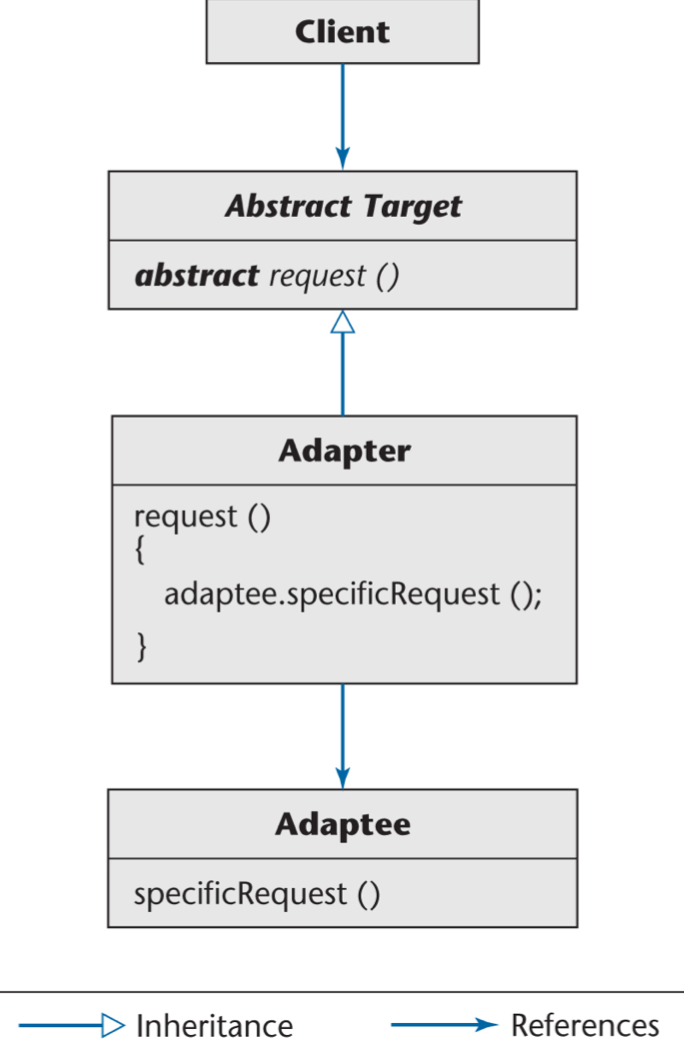
\includegraphics[width=0.5\linewidth]{images/AdapterPattern.png}
	\caption{Adapter Design Pattern}
	\label{fig:AdapterPattern}
\end{figure}

\section*{Bridge Design Pattern}

The Bridge design pattern aims to decouple an abstraction from its implementation so that the two can be changed independently of one another. Sometimes it's also called a \textit{driver}.

\begin{figure}[h]
	\centering
	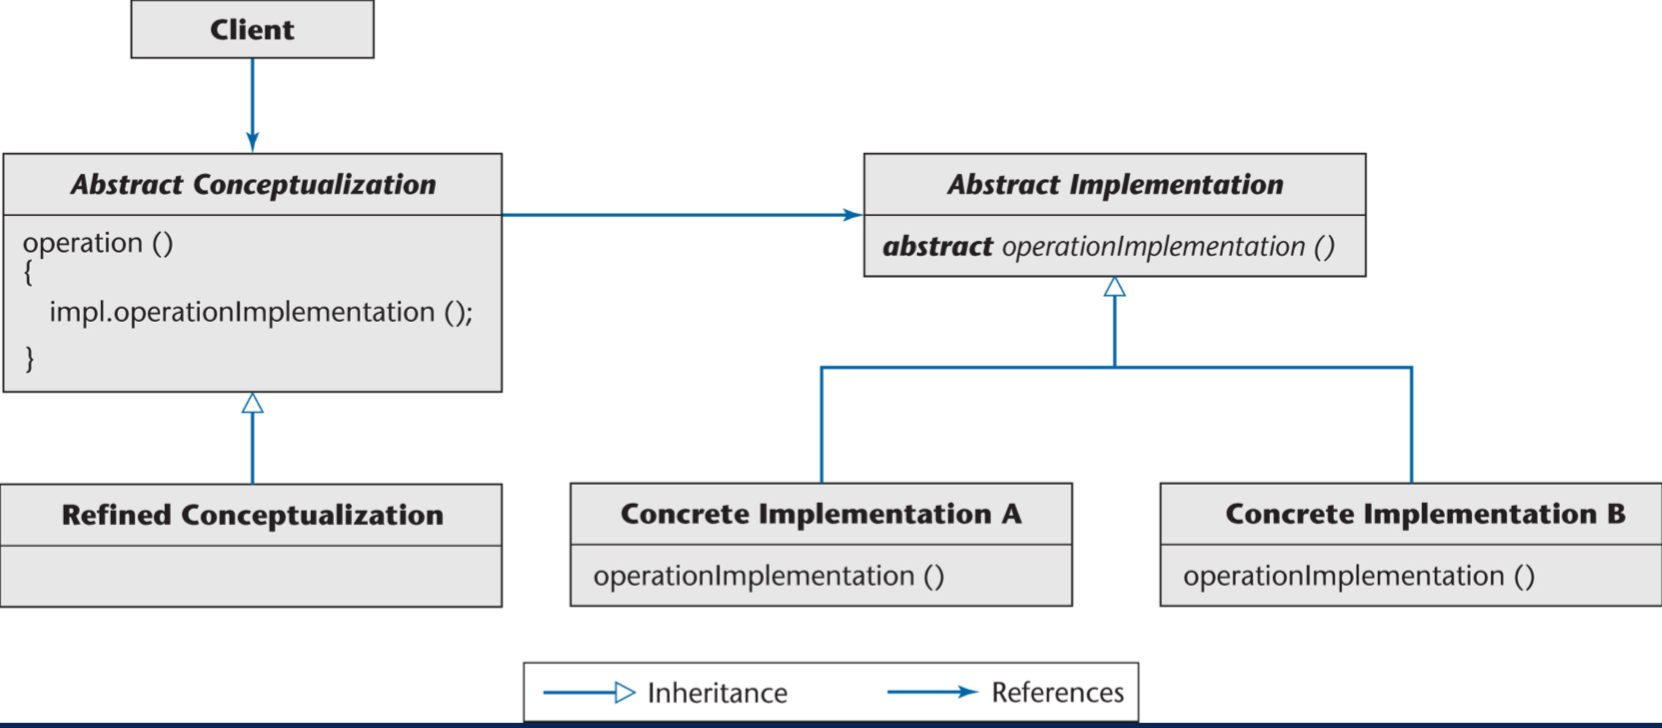
\includegraphics[width=0.9\linewidth]{images/BridgePattern.png}
	\caption{Bridge Design Pattern}
	\label{fig:BridgePattern}
\end{figure}

\section*{Iterator Design Pattern}

An aggregate object (or container or collection) is an object that contains other objects grouped together as a unit. An iterator (or cursor) is a programming construct that allows a programmer to traverse the elements of an aggregate object without exposing the implementation of that aggregate.

\begin{figure}[h]
	\centering
	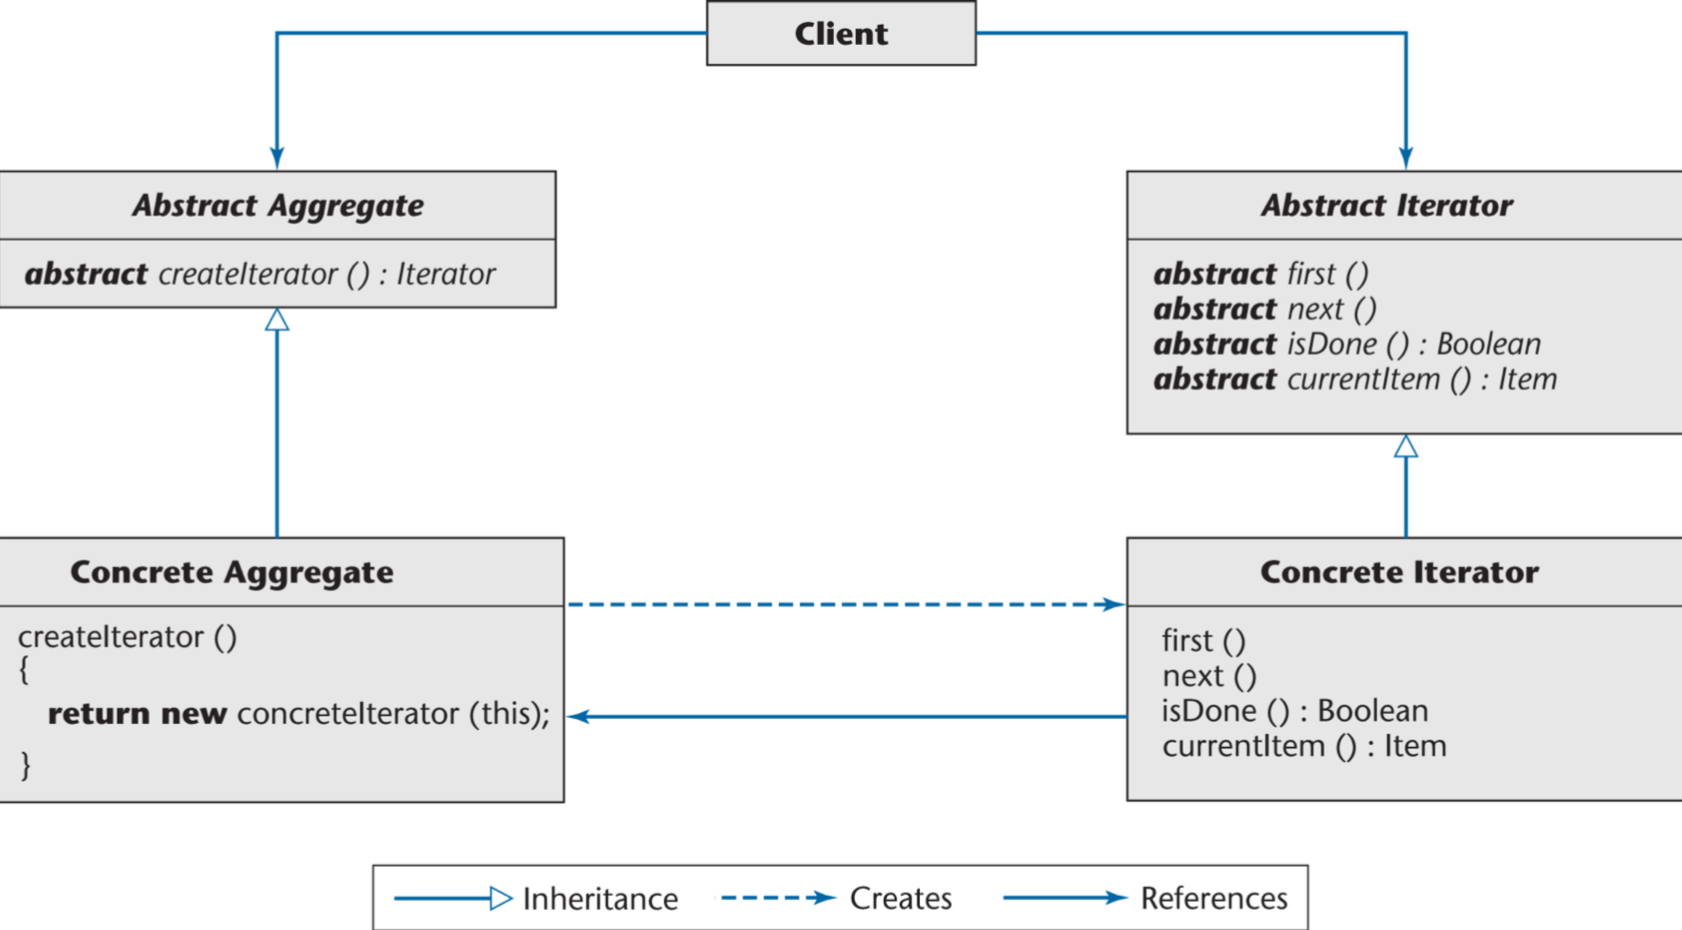
\includegraphics[width=0.9\linewidth]{images/IteratorPattern.png}
	\caption{Iterator Design Pattern}
	\label{fig:IteratorPattern}
\end{figure}

\newpage
\section*{Abstract Factory Design Pattern}
\begin{figure}[h]
	\centering
	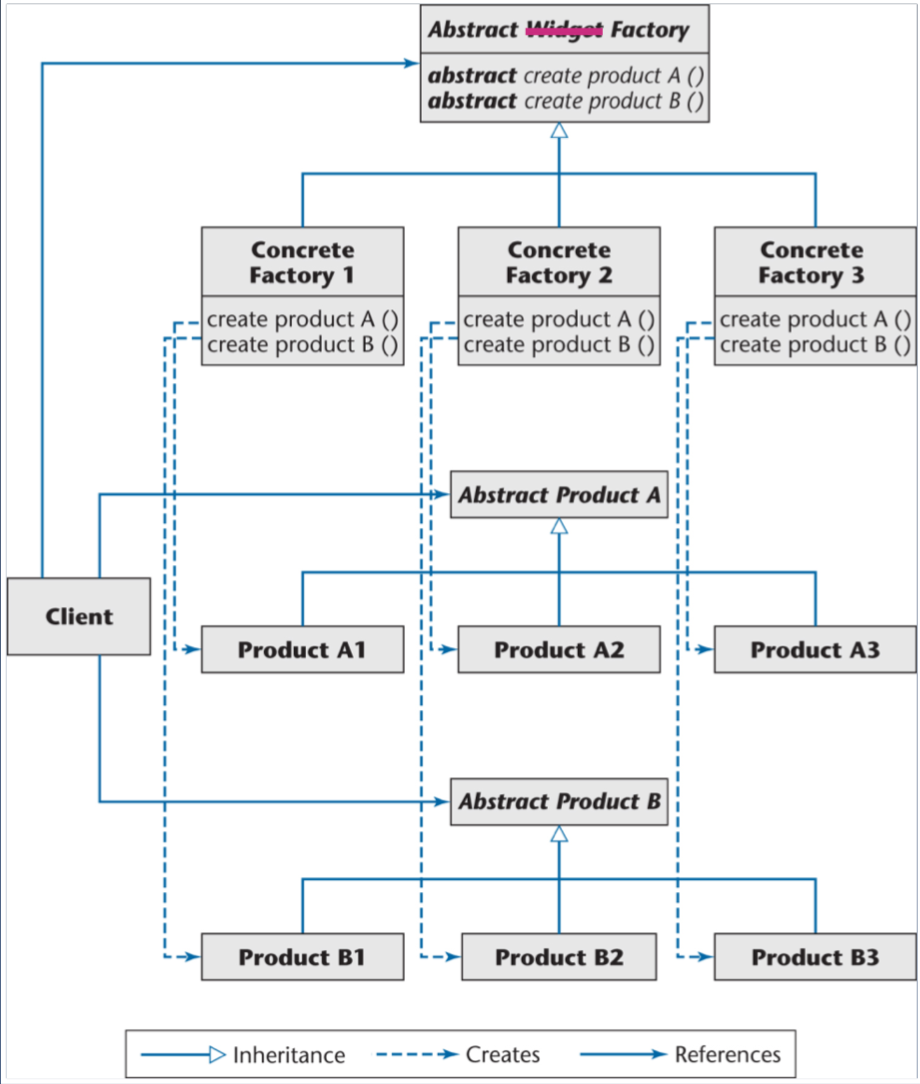
\includegraphics[width=0.9\linewidth]{images/AbstractFactoryPattern.png}
	\caption{Abstract Factory Pattern}
	\label{fig:AbstractFactoryPattern}
\end{figure}

\newpage
\section*{Categories of Design Patterns}
\begin{itemize}

	\item \textbf{Creational Design Patterns}
	
	Creational design patterns solve design problems by creating objects.
	\begin{figure}[h]
		\centering
		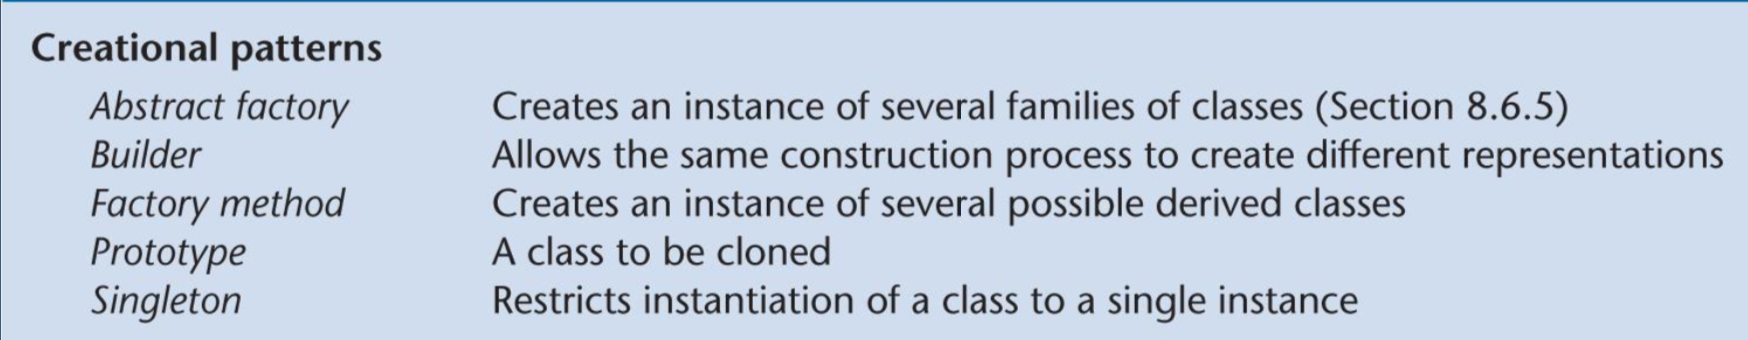
\includegraphics[width=0.84\linewidth]{images/CreationalPattern.png}
		\caption{Creational Design Pattern}
		\label{fig:CreationalPattern}
	\end{figure}
	
	\item \textbf{Structural Design Patterns}
	
	Structural design patterns solve design problems by identifying a simple way to realize relationships between entities.
	\begin{figure}[h]
		\centering
		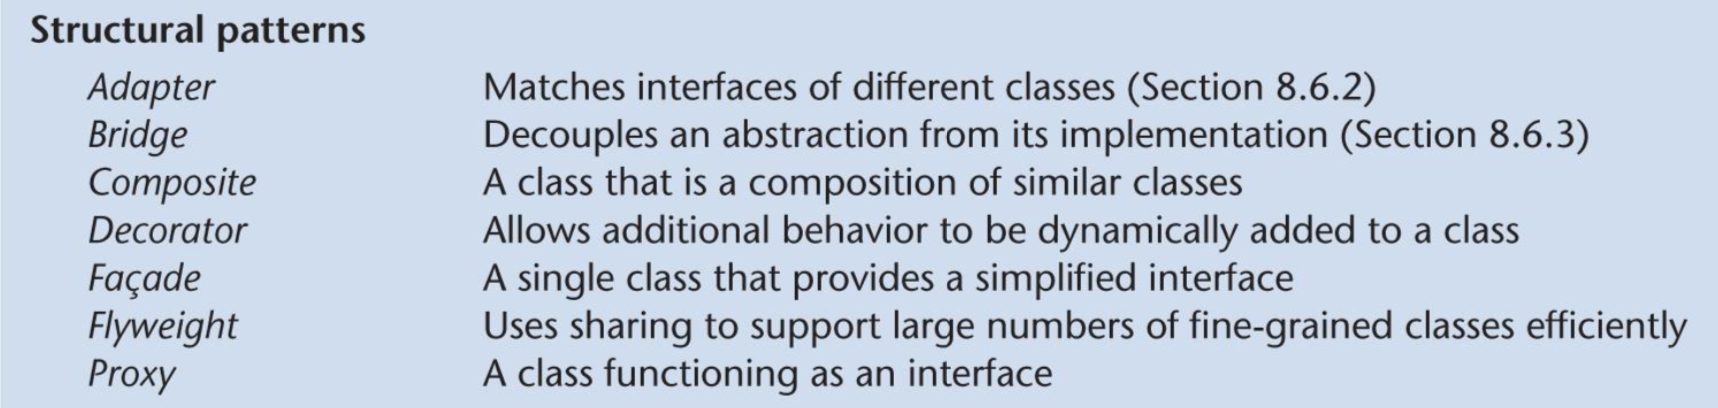
\includegraphics[width=0.84\linewidth]{images/StructuralPattern.png}
		\caption{Structural Design Pattern}
		\label{fig:StructuralPattern}
	\end{figure}
	
	\item \textbf{Behavioral Design Patterns}
	
	Behavioral design patterns solve design problems by identifying common communication patterns.
	\begin{figure}[h]
		\centering
		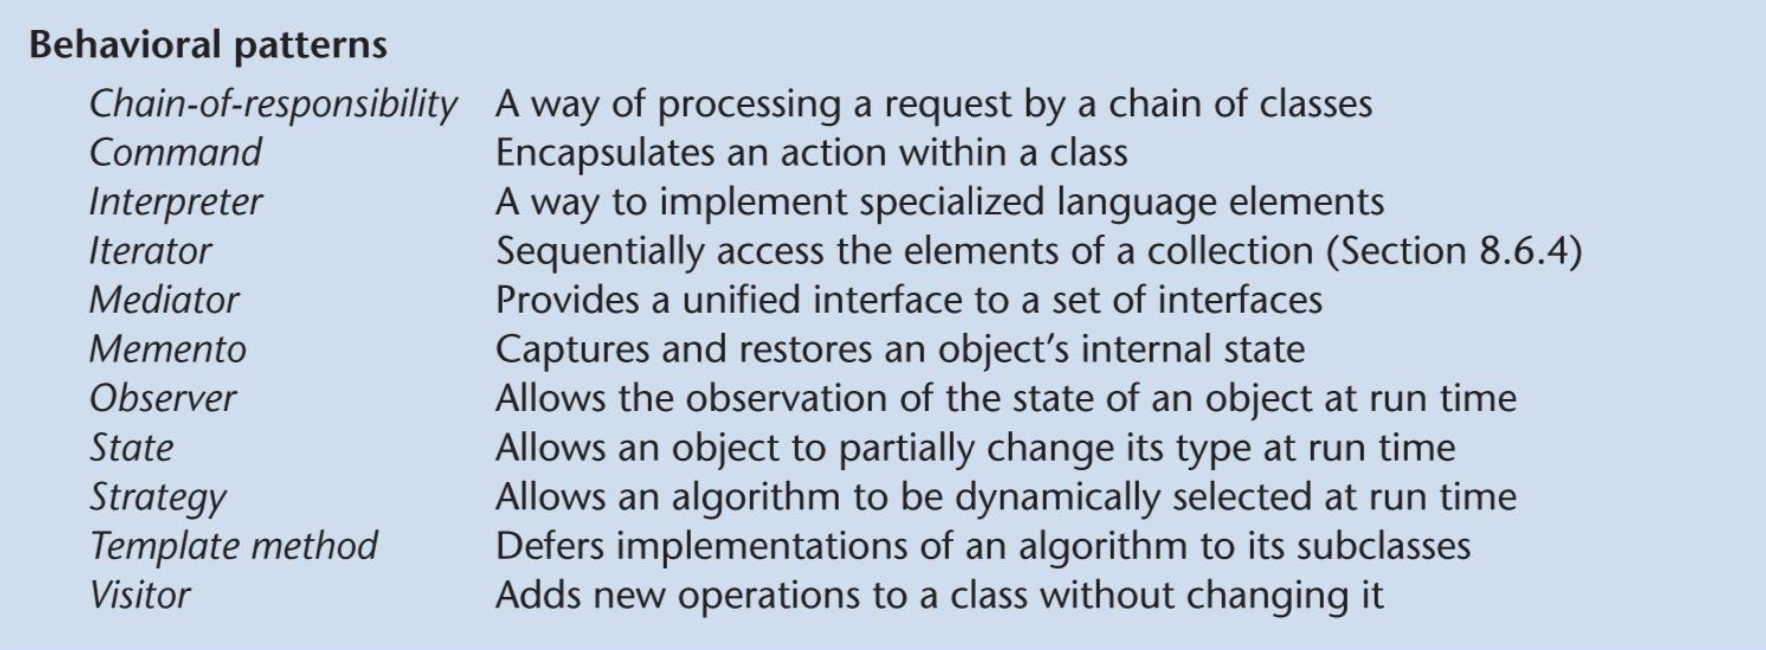
\includegraphics[width=0.84\linewidth]{images/BehavioralPattern.png}
		\caption{Behavioral Design Pattern}
		\label{fig:BehavioralPattern}
	\end{figure}

	
\end{itemize}




\end{document}